\begin{name}
	{\tenchude}
	{TOÁN 10}
	{LỚP TOÁN THẦY PHÁT}
	{Thời gian: 90 phút - Không kể thời gian phát đề}
\end{name}
\Opensolutionfile{ansbook}[ans/ansbookDe3]
\TN
\Opensolutionfile{ans}[ans/ansDe3-TN1]
\begin{ex}%[Mức 2]%[0D3H1-5]
	Xét sự biến thiên của hàm số $f(x)=\dfrac{3}{x}$ trên khoảng $(0 ;+\infty)$. Khẳng định nào sau đây đúng?
	\choice
	{\True Hàm số nghịch biến trên khoảng $(0 ;+\infty)$}
	{ Hàm số vừa đồng biến, vừa nghịch biến trên khoảng $(0 ;+\infty)$}
	{Hàm số đồng biến trên khoảng $(0 ;+\infty)$}
	{Hàm số không đồng biến, không nghịch biến trên khoảng $(0 ;+\infty)$}
	\loigiai
	{
		Ta có $f(x_1)-f(x_2)=\dfrac{3}{x_1}-\dfrac{3}{x_2}=\dfrac{3(x_2-x_1)}{x_1x_2}=-\dfrac{3(x_1-x_2)}{x_1x_2}$\\
		Với mọi $x_1$, $x_2\in (0 ;+\infty) $ và $x_1 < x_2$.\\
		Ta có $ \heva{x_1>0\\x_2>0} \Rightarrow x_1 \cdot x_2 >0$\\
		Suy ra $ \dfrac{f(x_1)-f(x_2)}{x_1-x_2}=-\dfrac{3}{x_1x_2}<0 \Rightarrow f(x)$ nghịch biến trên $(0 ;+\infty)$.
	}
\end{ex}

\begin{ex}%[24-25 giảng K10 - K11, Phan Quốc Trí]%[0D3N2-1]
	Trong các hàm số sau, hàm số nào là hàm số bậc hai?
	\choice
	{\True $y=2x^2-3x+4$}
	{$y=-x^2+2x+\dfrac{1}{x}$}
	{$y=1-3x$}
	{$y=x^2+\sqrt{2x}-x^3$}
	\loigiai{
		Từ các phương án đã cho, ta thấy hàm số bậc hai là $y=2x^2-3x+4$.
	}
\end{ex}

\begin{ex}%[Mức độ 2]%[24-25 Bai giang K10-K11, Phạm Ngọc Trung]%[0D3H2-2]
	Giá trị nhỏ nhất của hàm số $y=x^2-4x+1$ là
	\choice
	{\True $-3$}
	{$1$}
	{$3$}
	{$13$}
	\loigiai
	{
		Ta có $x^2-4x+1=x^2-4x+4-3=(x-2)^2-3\geqslant-3$. \\
		Dấu \lq\lq$=$\rq\rq\ xảy ra khi $x=2$. \\
		Vậy giá trị nhỏ nhất của hàm số $y=x^2-4x+1$ bằng $-3$ khi $x=2$.
	}
\end{ex}

\begin{ex}%[10-11-GK2-2425]%[Đỗ Minh Phúc]%[0D6H1-1]
	Cho giá trị gần đúng của $\dfrac{5}{12}$ là $0{,}417$. Sai số tuyệt đối của số $0{,}417$ gần với đáp án nào nhất.
	\choice
	{$0{,}003$}
	{\True $0{,}0003$}
	{$0{,}00003$}
	{$-0{,}0003$}
	\loigiai{
	Sai số tuyệt đối là $\Delta_a=\left|\dfrac{5}{12}-0{,}417\right|\approx 0{,}0003$.
	}
\end{ex}

\begin{ex}%[H]%[BG10-3in1, Phạm Ngọc Trung]%[0D6H4-2]
	\immini{
		Biểu đồ đoạn thẳng ở hình bên biểu diễn giá vàng bán ra trong bảy ngày đầu tiên của tháng $6$ năm $2021$. Tìm khoảng tứ phân vị của mẫu số liệu.
		\choice[1]
		{$29$}
		{\True $30$}
		{$31$}
		{$32$}
	}
	{\color{blue}
		\begin{tikzpicture}[scale=0.8, font=\footnotesize, line join=round, line cap=round, >=stealth]
			\draw[->,>=stealth,line width=1.5] (0,0)--(0,6); \draw[->,>=stealth,line width=1.5] (0,0)--(8.5,0);
			\path
			(-0.6,0) node {$5 710$}
			(-0.6,1.1) node {$5 722$}
			(-0.6,1.5) node {$5 727$}
			(-0.6,2.5) node {$5737$}
			(-0.6,3.5) node {$5747$}
			(-0.6,4.5) node {$5757$}
			(-0.6,5.5) node {$5767$}
			(0,6.4) node {Giá vàng (nghìn đồng/chỉ)}

			(1,-0.5) node {$1/6$}
			(2,-0.5) node {$2/6$}
			(3,-0.5) node {$3/6$}
			(4,-0.5) node {$4/6$}
			(5,-0.5) node {$5/6$}
			(6,-0.5) node {$6/6$}
			(7,-0.5) node {$7/6$}
			(8.2,-0.5) node {Ngày};

			\draw[line width=1.5,red] (1,5.5)--(2,4.5)--(3,2.5)--(4,1.5)--(5,3.5)--(6,3.5)--(7,1.2);
			\draw[dashed] (0,5.5)--(1,5.5)--(1,0) (0,4.5)--(2,4.5)--(2,0) (0,2.5)--(3,2.5)--(3,0) (0,1.5)--(4,1.5)--(4,0) (0,3.5)--(5,3.5)--(5,0) (6,3.5)--(6,0) (0,1.2)--(7,1.2)--(7,0);
			\fill[black] (1,5.5) circle (2.5pt);
			\fill[black] (2,4.5)circle (2.5pt);
			\fill[black] (3,2.5)circle (2.5pt);
			\fill[black] (4,1.5)circle (2.5pt);
			\fill[black] (5,3.5)circle (2.5pt);
			\fill[black] (6,3.5)circle (2.5pt);
			\fill[black] (7,1.2) circle (2.5pt);
		\end{tikzpicture}
	}
	\loigiai{
		\begin{itemize}
			\item 	Mẫu số liệu thống kê tốc độ tăng trưởng GDP nhận được
			      \begin{center}
				      \begin{tabular}{|c|c|c|c|c|c|c|c|}
					      \hline
					      Ngày                      & $1/6$  & $2/6$  & $3/6$  & $4/6$  & $5/6$  & $6/6$  & $7/6$  \\
					      \hline
					      Giá vàng (nghìn đồng/chỉ) & $5767$ & $5757$ & $5737$ & $5727$ & $5747$ & $5747$ & $5722$ \\
					      \hline
				      \end{tabular}\\
				      Sắp xếp lại mẫu số liệu ta được \\
				      \begin{tabular}{cccccccc}
					       & $5722$ & $5727$ & $5737$ & $5747$ & $5747$ & $5757$ & $5767$
				      \end{tabular}
			      \end{center}
			\item
			      Ta có $Q_2=5747; \; Q_1=5727; \; Q_3=5757$.\\
			      Vậy khoảng tứ phân vị $\Delta_Q=Q_3-Q_1=5757-5727=30$.
		\end{itemize}
	}
\end{ex}

\begin{ex}%[0D0N1-2]
	Tung một đồng xu và một con súc sắc, nhận được kết quả là mặt xuất hiện trên đồng xu (sấp hay ngửa) và số chấm xuất hiện trên con súc sắc. Số kết quả có thể xảy ra là
	\choice
	{$2$}
	{$6$}
	{$8$}
	{\True $12$}
	\loigiai{
		Đồng xu chỉ có hai mặt sấp hay ngửa.\\
		Con súc sắc số chấm xuất hiện là $1,2,3,4,5,6$.\\
		Số kết quả có thể xảy ra là $2\cdot 6=12$.
	}
\end{ex}

\begin{ex}%[0D0N1-3]
	Gieo một đồng tiền và một con súc sắc. Số phần tử của không gian mẫu là
	\choice
	{$24$}
	{\True $12$}
	{$6$}
	{$8$}
	\loigiai{
		Mô tả không gian mẫu ta có $\Omega=\{S1; S2; S3; S4; S5;S6;N1;N2;N3;N4;N5;N6\}$.
	}
\end{ex}

\begin{ex} %[0H9N3-1]
	Trong mặt phẳng $O x y$, cho đường thẳng $\Delta$ có phương trình $\dfrac{x-1}{2}=\dfrac{y+1}{-1}$. Véctơ chỉ phương của đường thẳng $\Delta$ là
	\choice
	{\True $\vec{u}(2 ;-1)$}
	{$\vec{u}(1 ; 2)$}
	{$\vec{u}(1 ;-1)$}
	{$\vec{u}(1 ; 1)$}
	\loigiai{
		Từ phương trình đường thẳng $\Delta$ suy ra véctơ chỉ phương của đường thẳng $\Delta$ là $\vec{u}(2 ;-1)$.
	}
\end{ex}

\begin{ex}
	Trong mặt phẳng $Oxy$, khoảng cách từ điểm $A(x_0;y_0)$ đến đường thẳng $\Delta \colon ax+by+c=0$ được tính bằng công thức
	\choice
	{$d=\dfrac{|ax_0+by_0+c|}{\sqrt{a^2+b^2}}$}
	{$d=\dfrac{|ax_0+by_0-c|}{\sqrt{a^2+b^2}}$}
	{\True $d=\dfrac{|ax_0+by_0+c|}{\sqrt{a^2+b^2}}$}
	{$d=\dfrac{|ax_0-by_0+c|}{\sqrt{a^2+b^2}}$}
	\loigiai{
		Ta có công thức tính khoảng cách từ điểm $A(x_0;y_0)$ đến đường thẳng $\Delta \colon ax+by+c=0$ là
		$d=\dfrac{|ax_0+by_0+c|}{\sqrt{a^2+b^2}}.$
	}
\end{ex}

\begin{ex}%[0H9N3-3]
	Cho hai đường thẳng $\Delta_1\colon \sqrt{7}x-2y-3=0$ và $\Delta_2\colon 2x-\sqrt{7}y+3=0$. Vị trí tương đối của $2$ đường thẳng này là
	\choice
	{\True $\Delta_1$ cắt $\Delta_2$}
	{$\Delta_1$ song song $\Delta_2$}
	{$\Delta_1$ trùng $\Delta_2$}
	{$\Delta_1$ cắt $\Delta_2$ và $\Delta_1 \perp \Delta_2$}
	\loigiai{
		Ta có $\heva{&\Delta_1\colon \sqrt{7}x-2y-3=0\\ &\Delta_2\colon 2x-\sqrt{7}y+3=0}\Leftrightarrow \heva{&x=2+\sqrt{7}\\ &y=2+\sqrt{7}.}$\\
		Vì $\overrightarrow{n}_{\Delta_1}\cdot\overrightarrow{n}_{\Delta_2}=\sqrt{7}\cdot2+(-2)\cdot\left(-\sqrt{7}\right)=4\sqrt{7}\neq0$.\\
		Nên $\Delta_1$ cắt $\Delta_2$ nhưng không vuông góc.
	}
\end{ex}

\begin{ex}%[0H9N5-1]%[Dự án đề kiểm tra Toán Khối 10 CK2 NH23-24-Dot 16- Khắc Thiên]%[THPT Chuyên Hùng Vương - Phú Thọ]
	Trong mặt phẳng $Oxy$, cho đường elip $(E)$ có phương trình  $\dfrac{x^2}{36}+\dfrac{y^2}{9}=1$. Tổng khoảng cách từ mỗi điểm trên elip tới hai tiêu điểm bằng
	\choice
	{$6$}
	{$3$}
	{$5$}
	{\True $12$}
	\loigiai{
		Ta có phương trình của chính tắc elip  $(E)$ là $\dfrac{x^2}{36}+\dfrac{y^2}{9}=1$.\\
		Suy ra $a=6$.\\
		Khi đó, tổng khoảng cách từ mỗi điểm trên elip tới hai tiêu điểm bằng $2a=12$.
	}
\end{ex}

\begin{ex}%[0H9N5-5]%[Dự án đề kiểm tra Toán Khối 10 CK2 NH23-24-Dot 16- Khắc Thiên]%[THPT Chuyên Hùng Vương - Phú Thọ]
	Phương trình nào sau đây là phương trình chính tắc của hypebol?
	\choice
	{$\dfrac{x^2}{9}+\dfrac{y^2}{4}=1$}
	{$\dfrac{x^2}{4}-\dfrac{y^2}{9}=-1$}
	{\True $\dfrac{x^2}{4}-\dfrac{y^2}{9}=1$}
	{$\dfrac{x^2}{9}+\dfrac{y^2}{9}=1$}
	\loigiai{
		Phương trình chính tắc của hypebol có dạng $\dfrac{x^2}{a^2}-\dfrac{y^2}{b^2}=1$ (với $a>0$, $b>0$) nên $\dfrac{x^2}{4}-\dfrac{y^2}{9}=1$ là  phương trình chính tắc của hypebol.
	}
\end{ex}
\Closesolutionfile{ans}

\TNTF
\Opensolutionfile{ans}[ans/ansDe3-TN2]
\begin{ex}%[0D6H4-2]%[Dự án đề kiểm tra Toán 11 GHKII NH23-24- Hieu Hieu Minh Minh]%[THPT Toàn Thắng- Hải Phòng]
	Điều tra về chiều cao (đơn vị: $\mathrm{cm}$ ) của $12$ học sinh tổ $1$ lớp $10 \mathrm{C}$ thu được bảng số liệu sau: \[\begin{array}{llllllllllll}
			154 & 150 & 152 & 160 & 165 & 168 & 154 & 170 & 163 & 172 & 152 & 160
		\end{array}\]
	Khi đó:
	\choiceTF
	{Mẫu số liệu có khoảng tứ phân vị là $6 \mathrm{cm}$}
	{\True Độ chênh lệch chiều cao tối đa của các học sinh là $22 \mathrm{cm}$}
	{\True Quy tròn phương sai của mẫu số liệu với độ chính xác $d=0,5$ là $54$}
	{\True Sai số tương đối của số quy tròn phương sai trên xấp xỉ $0,9\%$}
	\loigiai{
		\begin{itemchoice}
			\itemch Sai.
			\begin{itemize}
				\item Nửa số liệu bên trái là $150$; $152$; $152$; $154$; $154$; $160$ gồm  $6$  giá trị nên $Q_1=153$.
				\item  Nửa số liệu bên phải là $160$; $163$; $165$; $168$; $170$; $172$ gồm  $6$  giá trị nên $Q_3=166{,}5$.
			\end{itemize}
			Do đó khoảng tứ phân vị của mẫu số liệu bằng $\Delta_Q=Q_3-Q_1=166{,}5-160=6{,}5$.
			\itemch Đúng. Chiều cao nhỏ nhất là $150 \mathrm{cm}$ và chiều cao lớn nhất là $172\mathrm{cm}$ nên độ chênh lệch chiều cao tối đa của các học sinh là $22\mathrm{cm}$.
			\itemch Sai.\\
			Sử dụng máy tính bỏ túi ta được phương sai mẫu là $53,5$.\\
			Vậy quy tròn phương sai của mẫu số liệu với độ chính xác $d=0,5$ là $54$.
			\itemch Sai.\\
			Sai số tương đối của số quy tròn phương sai là
			\[\delta=\dfrac{54-53,5}{54}\approx 0,009\approx 0,9\%.\]
		\end{itemchoice}
	}
\end{ex}

\begin{ex}%[0H9H3-2]%[0H9H3-3]
	Trong mặt phẳng tọa độ $Oxy$, cho đường thẳng $d_1\colon x-2y+3=0$; $d_2\colon 3x-y-1=0$ và điểm $A(2;1)$.
	\choiceTF
	{Đường thẳng đi qua $A$ và song song với $d_1$ có phương trình $2x+y-5=0$}
	{\True Hai đường thẳng $d_1$ và $d_2$ cắt nhau tại điểm $M(1;2)$}
	{Phương trình đường tròn tâm $A$ đi qua $M$ là $(x-2)^2+(y-1)^2=5$}
	{Tiếp tuyến của đường tròn $(A)$ tại $M$ có phương trình $x-2y+1=0$}
	\loigiai{
		\begin{itemchoice}
			\itemch {\bf Sai}.\\
			Gọi $\Delta_1$ là đường thẳng song song với $d_1$.\\
			Suy ra $\Delta_1$ có phương trình dạng $x-2y+c=0$.\\
			Mặt khác, $\Delta_1$ đi qua $A(2;1)$ suy ra $2-2\cdot 1+c=0\Rightarrow c=0$.\\
			Vậy, đường thẳng đi qua $A$ và song song với $d_1$ có phương trình $x-2y=0$.
			\itemch {\bf Đúng}.\\
			Giao điểm của $d_1$ và $d_2$ là nghiệm của hệ phương trình $\heva{&x-2y+3=0\\&3x-y-1=0.}$\\
			Giải hệ ta được $\heva{&x=1\\&y=2.}$\\
			Vậy, hai đường thẳng $d_1$ và $d_2$ cắt nhau tại điểm $M(1;2)$.
			\itemch {\bf Sai}.\\
			Đường tròn $(A)$ có tâm $A(2;1)$ và đi qua $M(1;2)$ nên có bán kính $R=AM=\sqrt{(2-1)^2+(1-2)^2}=\sqrt{2}$.\\
			Vậy, phương trình đường tròn $(A)$ là $(x-2)^2+(y-1)^2=2$.
			\itemch {\bf Sai}.\\
			Ta có phương trình tiếp tuyến của đường tròn $(A)$ tại điểm $M(1;2)$ là
			\[(x-2)(1-2)+(y-1)(2-1)=0\Leftrightarrow (x-2)+y-1=0\Leftrightarrow x+y-3=0.\]
		\end{itemchoice}
	}
\end{ex}
\Closesolutionfile{ans}

\TNSA
\Opensolutionfile{ans}[ans/ansDe3-TN3]
\begin{ex}%[Mức 2]%[24-25 giảng K10-K11, Nguyễn Xuân Bảo]%[0D3H2-3]
	Cho đồ thị $(P)\colon y=a x^{2}+b x+2,$ biết rằng $(P)$ đi qua $M(1 ; 5)$ và $N(-2 ; 8)$. Tính $a+b$.
	\shortans{$3$}
	\loigiai{
		Parabol $(P)\colon y=a x^{2}+b x+2,$ biết rằng $(P)$ đi qua $M(1 ; 5)$ và $N(-2 ; 8)$		khi đó
		\[\heva{&a+b+2=5\\&4a-2b+2=8}\Leftrightarrow\heva{&a+b=3\\&4a-2b=6}\Leftrightarrow \heva{&a=2\\&b=1.}\]
		Vậy $a+b=3$.
	}
\end{ex}

\begin{ex}%[10-11-12EX-HK1-2425]%[Trương Quan Kía]%[0D7V2-7]
	Tổng chi phí $P$ (đơn vị$\colon$ nghìn đồng) để sản xuất $x$ sản phẩm được biểu diễn bởi biểu thức $P = x^2 + 30x + 3\,000$. Giá bán một sản phẩm là $160$ nghìn đồng. Số sản phẩm được sản xuất trong đoạn $[a; b]$ để đảm bảo nhà sản xuất không bị lỗ (giả sử các sản phẩm được bán hết). Giá trị $a + b$ bằng bao nhiêu?
	\shortans[oly]{$130$}
	\loigiai{
		Nhà sản xuất không bị lỗ khi doanh thu lớn hơn hoặc bằng tổng chi phí.\\
		Doanh thu là $R(x)=160x$, tổng chi phí là $P(x)=x^2+30x+3\,000$.\\
		Theo bài toán ta suy ra $160x\ge x^2+30x+3\,000\Leftrightarrow x^2-130x+3\,000\le 0\Leftrightarrow x\in[30;100]$.\\
		Vậy để không bị lỗ thì $x\in[30;100]\Rightarrow a=30,b=100$.\\
		Suy ra $a+b=30+100=130$.
	}
\end{ex}

\begin{ex}%[De-chuan-hoa-so-8]%[Duong Xuan Loi]%[0D6H3-2]
	Bảng dưới đây thống kê nhiệt độ (đơn vị: ${}^{\circ}{C}$) ở thành phố Hồ Chí Minh ngày $03 / 06 / 2021$ sau một số lần đo
	\begin{center}
		\begin{tabular}{|l|c|c|c|c|c|c|c|c|}
			\hline
			Giờ đo                                       & $1 $ h & $4 $ h & $7 $ h & $10 $ h & $13 $ h & $16 $ h & $19 $ h & $22 $ h \\
			\hline Nhiệt độ $\left({}^{\circ}{C}\right)$ & $27$   & $26$   & $28$   & $32$    & $34$    & $35$    & $30$    & $28$    \\
			\hline
		\end{tabular}
	\end{center}
	Tìm số trung bình của mẫu số liệu (làm tròn kết quả đến hàng phần trăm).
	\shortans{$30$}
	\loigiai{
		% Sắp xếp dãy số liệu nhiệt độ theo thứ tự không giảm ta được: $26;27;28;28;30;32;34;35$.\\
		Nhiệt độ trung bình $\overline{x}=\dfrac{26+27+28\cdot 2+30+32+34+35}{8}=30$.\\
		% Số trung vị $M_e=\dfrac{28+30}{2}=29$.
	}
\end{ex}

\begin{ex}%[0H9V4-2]
	Trong mặt phẳng với hệ tọa độ $Oxy$, cho đường thẳng $d\colon 2x-y-5=0$ và hai điểm $A\left(1;2\right), B\left(4;1\right)$. Tính bán kính đường tròn $(C)$ có tâm thuộc $d$ và đi qua hai điểm $A, B$.
	\shortans{$5$}
	\loigiai{
		\immini{
			Gọi $I$ là tâm của $(C)$. Do $I\in d$ nên $I\left(t;2t-5\right)$.\\
			Hai điểm $A, B$ cùng thuộc $(C)$ nên
			\begin{align*}
				IA=IB & \Leftrightarrow (1-t)^2+\left(7-2t\right)^2=(4-t)^2+\left(6-2t\right)^2 \\
				      & \Leftrightarrow t=1.
			\end{align*}
			Suy ra $I(1;-3)$ và bán kính $R=IA=5$.\\

		}
		{
			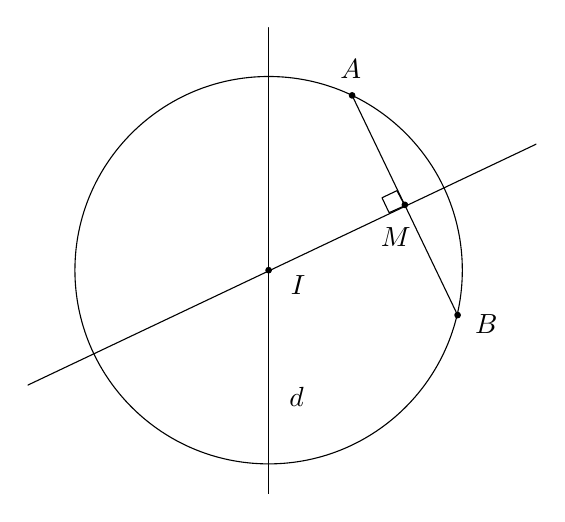
\begin{tikzpicture}[line cap=round,line join=round,>=stealth,x=1.0cm,y=1.0cm]
				\clip(1.24,-1.) rectangle (7.7,4.92);
				\draw (5.93,2.85) -- (5.74,2.76) -- (5.83,2.57) -- (6.03,2.66) -- cycle;
				\draw (4.3,1.84) circle (2.46cm);
				\draw (5.36,4.06)-- (6.7,1.27);
				\draw [domain=1.24:7.7] plot(\x,{(-0.36--0.82*\x)/1.73});
				\draw (4.3,-1.) -- (4.3,4.92);
				\draw (5.6,4.4) node[left] {$A$};
				\draw (6.8,1.4) node[anchor=north west] {$B$};
				\draw (5.6,2.5) node[anchor=north west] {$M$};
				\draw (4.44,0.48) node[anchor=north west] {$d$};
				\draw (4.46,1.9) node[anchor=north west] {$I$};
				\draw [fill=black] (4.3,1.84) circle (1.0pt);
				\draw [fill=black] (5.36,4.06) circle (1.0pt);
				\draw [fill=black] (6.7,1.27) circle (1.0pt);
				\draw [fill=black] (6.03,2.67) circle (1.0pt);
			\end{tikzpicture}
		}
	}
\end{ex}

\Closesolutionfile{ans}

\TL
\begin{ex}%[0D3H1-2]%[Đề cương Nguyễn Thượng Hiền]%[Mui Doan,DA3-ĐC-NTH-T10]
	Tìm tập xác định của các hàm số sau $y=\dfrac{2x+1}{\sqrt{x-2}\left(x^2-4x+3\right)}$.
	\loigiai{
		Điều kiện $\heva{&x-2>0 \\ x^2-4x+3 \ne 0}\Leftrightarrow \heva{&x>2\\&x\neq 1\\&x\neq 3.}$\\
		Tập xác định $\mathscr{D}=(2;+\infty)\setminus\left\{3\right\}$.
	}
\end{ex}


\begin{ex}%[0D7C3-6]
	Người ta làm ra một cái thang bắc lên tầng hai của một ngôi nhà (tham khảo hình vẽ).
	\begin{center}
		\begin{tikzpicture}[scale=1, font=\footnotesize, line join=round, line cap=round, >=stealth]
			\def\h{4} \def\rt{.03}
			\path (0,0) coordinate (A) (0:2) coordinate (B)++(0:3)coordinate (D)++(90:\h)coordinate (E)
			(B)++(90:1)coordinate (Bt)
			(intersection of A--E and B--Bt) coordinate (C);
			\fill[pattern=bricks,pattern color=brown ] (D) rectangle (6.5,\h+.6);
			\draw (A)--(D)--(E)--cycle (B)--(C)node[right,pos=.5]{$4m$};
			\foreach \p/\g in {A/180,B/-90,C/90,D/-90,E/180} \fill[black] (\p) circle(1pt)+(\g:0.25) node{$\p$};
		\end{tikzpicture}
	\end{center}
	Muốn vậy họ cần làm một thanh đỡ $BC$ có chiều dài bằng $4$ m, đồng thời muốn đảm bảo kỹ thuật thì tỉ số độ dài $\dfrac{CE}{BD}=\dfrac{5}{3}$. Hỏi vị trí $A$ cách vị trí $B$ bao nhiêu mét?
	% \shortans{$3$}
	\loigiai{
		Đặt $AB=x > 0$.\\
		Xét tam giác $ABC$ vuông tại $B$ có $AC=\sqrt{x^2+4}$.\\
		Theo định lí Ta-lét, ta có
		\allowdisplaybreaks
		\begin{eqnarray*}
			&&\dfrac{AC}{AB}=\dfrac{CE}{BD}\\
			&\Leftrightarrow& \dfrac{\sqrt{x^2+16}}{x}=\dfrac{5}{3}\\
			&\Leftrightarrow& 3\sqrt{x^2+16}=5x\\
			&\Leftrightarrow& \heva{&5x\ge 0 \\	&9(x^2+16)=25x^2}\\
			&\Leftrightarrow& \heva{&x\ge 0 \\&16x^2=144}\\
			&\Leftrightarrow& x=3.
		\end{eqnarray*}
		Vậy hai vị trí $A$, $B$ cách nhau $3$ m.
	}
\end{ex}

\begin{ex}%[0D0C2-7]
	Gọi $S$ là tập hợp tất cả các số có $5$ chữ số khác nhau được lập từ các chữ số $0,1,2,3,4,5,6,7$. Chọn ngẫu nhiên một số từ $S$. Tính xác suất để số chọn được chia hết cho $5$, luôn có mặt các chữ số $2,3,4$ và chúng đứng cạnh nhau (kết quả làm tròn đến hai số thập phân).
	% \shortans{$0{,}02$}
	\loigiai{
		Ta có $n\left(\Omega \right)=7\cdot \mathrm{A}_7^4=5880$.\\
		Ta tính số các số chia hết cho $5$, luôn có mặt các chữ số $2,3,4$ và chúng đứng cạnh nhau.\\
		Xếp các chữ số $2,3,4$ thành một nhóm, coi là một chữ số, có $3!=6$ cách.\\
		Do đó: ta cần tính số các số có $3$ chữ số đôi một khác nhau từ các chữ số $0,1,(234),5,6,7$ sao cho số đó chia hết cho $5$, và luôn có mặt nhóm $(234)$.\\
		Vì số đó chia hết cho $5$ nên chữ số hàng đơn vị bằng $0$ hoặc $5$, có $2$ cách chọn.\\
		Chọn vị trí cho nhóm $(234)$, có $2$ cách chọn.\\
		Viết chữ số còn lại, có $4$ cách chọn.\\
		Suy ra: số các số cần tìm là: $2.2.4=16$ số.\\
		Trong các số đó, có một số không thỏa mãn là $0(234)5$.\\
		Do đó, các số các số có $3$ chữ số đôi một khác nhau từ các chữ số $0,1,(234),5,6,7$ thỏa mãn yêu cầu là: $16-1=15$.\\
		Vậy số các số có $5$ chữ số thỏa mãn yêu cầu đề bài là: $6\cdot 15=90$ số.\\
		Vậy xác suất cần tìm là $\mathrm{P}=\dfrac{90}{5880}=\dfrac{3}{196} \approx 0{,}02$.
	}
\end{ex}
\Closesolutionfile{ansbook}
